\documentclass[conference]{IEEEtran}
\usepackage{cite}
\usepackage{amsmath,amssymb,amsfonts}
\usepackage{algorithmic}
\usepackage{algorithm}
\usepackage{graphicx}
\usepackage{textcomp}
\usepackage{hyperref}
\usepackage{subcaption}
\usepackage{xcolor}
\newcommand{\todo}[1]{\textcolor{red}{#1}}

\def\BibTeX{{\rm B\kern-.05em{\sc i\kern-.025em b}\kern-.08em
    T\kern-.1667em\lower.7ex\hbox{E}\kern-.125emX}}
\begin{document}


\title{Joint audio denoising and inpainting with plug-and-play proximal algorithm}

\author{\IEEEauthorblockN{Michal Švento}
\IEEEauthorblockA{
	\textit{Brno University of Technology, FEEC,} \\
	\textit{Department of Telecommunications,} \\
	Technická 12, 616 00 Brno, Czech Republic \\
	\href{mailto:212584@vut.cz}{212584@vut.cz}
}
\and
\IEEEauthorblockN{Ondřej Mokrý}
\IEEEauthorblockA{
	\textit{Brno University of Technology, FEEC,} \\
	\textit{Department of Telecommunications,} \\
	Technická 12, 616 00 Brno, Czech Republic \\
	\href{mailto:xmokry12@vut.cz}{xmokry12@vut.cz}
}
}

\maketitle

\begin{abstract}
We propose plug-and-play variant of the Douglas--Rachford proximal algorithm for audio inpainting, which replaces a proximal step with a denoiser.
In our situation, the observed samples are further degraded by noise.
We demonstrate that the plug-and-play aproach has potential to succeed in this joint task of inpainting and denoising.
Objective metrics show that the new method outperforms a conventional counterpart and that it is less sensitive to model hyperparameters.
\end{abstract}

\begin{IEEEkeywords}
speech enhancement, deep learning, denoising, Douglas--Rachford algorithm, inpainting
\end{IEEEkeywords}

\section{Introduction}

Audio enhancement tasks mostly face problems like missing or damaged samples, noise, or clipping.
Considering speech signals, 
we are not only interested in restoring the degradation sample by sample, but we also aim at improving the intelligibility of the recorded speech.
Each restoration problem has developed its own way of enhancing the signal.
Nowadays, the best way to differentiate algorithms is into two categories:
conventional, e.g.\ using autoregressive (AR) modeling or sparsity-based optimization, and solutions using deep learning.
The present paper focuses on the case of restoring a partially observed signal whose observed samples are further degraded by noise, i.e., the aim is to perform simultaneous inpainting and denoising of the speech signal.

In conventional approaches to inpainting, the AR-based Janssen \cite{Janssen1986} and Etter~\cite{Etter1996} algorithms dominate in terms of restoration quality.
A more recent, successful class of methods is based on sparsity.
The key idea is that after performing proper time-frequency analysis of an audio signal,
most of the information is concentrated in a few coefficients, i.e., it is sparse.
This can be applied as fitting the sparsest possible restoration either to the reliable observed samples \cite{Adler2012, Kitic2015, Zaviska2019, Mokry2019}, or to a signal not much diverging from the observation in the case of denoising \cite{Kowalski2013}.

Deep learning algorithms have also made their own progress in this area.
The most efficient neural network models are autoencoders,
recurrent neural networks (RNN) and
Generative Adversial Networks (GAN).
Current state-of-the-art deep learned algorithms are base on Speech Enhancement GAN (SEGAN) \cite{Pascual2017}, NSNet \cite{Xia2020}, FullSubNet \cite{Hao2021}.
While learning-based algorithms allow to adapt to real-world signals, rather than to rely on hand-crafted priors like sparsity or the AR nature of signals, they need large datasets for training.
Furthermore, neural networks are usually trained for a specific problem, lacking universal applicability on similar restoration tasks, in contrast to sparsity-based methods \cite{Gaultier2017, Mokry202021, Zaviska2021}.

As a compromise between the conventional and learning-based methods, 
the plug-and-play method for image restoration was introduced in \cite{Venkatakrishnan2013} and subsequently studied in \cite{Chan2016},
where part of each iteration of an optimization algorithm is replaced by a (learned) denoiser.
In the present paper, we propose a hybrid algorithm based on the same paradigm, aiming at restoration of degraded speech.
While \cite{Chan2016} focused on adapting the Alternating Direction method of Multipliers (ADMM) and a recent declipping approach used the learned element only partially \cite{Tanaka2022}, we choose an opposite approach by working with a simple Douglas--Rachford algorithm (DRA) and exploring the trade-off between data fitting and denoising in the algorithm.


The paper is organized as follows. In section \ref{sec:prereq} we introduce the task from mathematical point of view and we define the restoration as a minimization task.
Section \ref{sec:plugaandplay} presents the plug-and-play method and its challenges.
Section \ref{sec:eval} discusses the results and further improvements of algorithm.
Finally, Section \ref{sec:conclusion} concludes the paper.

\section{Prerequsities}\label{sec:prereq} 


In this section, we formalize the task of inpainting and denoising and propose algorithmic solutions based on DRA.
First, using frequency coefficients as input explained in \ref{subsec:freqcoef}~\cite{Mokry2020}.
Second, using samples in time domain is described in subsection \ref{subsec:timecoef} \cite{Mokry2021}.


\subsection{Task formulation}

We consider column vector $ \mathbf{s} \in \mathbb{R}^{N} $ as our observed damaged single-channel signal of length $ N $.
We have set % $ I $
of sample indices $ \{1,2,\dots,N\} $, which has two disjunctive subsets: $I_\textup{M} $ for missing positions and $ I_\textup{R} $ stands for reliable positions.
Usually, samples $ \mathbf{s}(I_\textup{R}) $ are considered reliable (undamaged) and $ \mathbf{s}(I_\textup{M}) $ are samples, which we are looking for.
It is common to rewrite it in matrix form:
\begin{equation*}
	\mathbf{s}_{\textup{R}} = \mathbf{M}_{\textup{R}}\mathbf{s},
\end{equation*}
where $\mathbf{M}_\textup{R} \in \mathbb{R} ^ { |I_\textup{R}| \times N}$ is the mask matrix, selecting rows from identity matrix corresponding to the indices in $I_\textup{R}$ \cite{Adler2012}, with $ |I_\textup{R}|$ denoting the number of indices in the subset $I_\textup{R}$.
In words, $\mathbf{M}_{\textup{R}}\mathbf{s}$ represents choosing the samples from $\mathbf{s}$ on positions $I_\textup{R}$.

It is convenient to define the set of signals fitting the observation as
\begin{equation}
	\label{eq:Gamma}
	\Gamma = \lbrace \mathbf{x}\in \mathbb {R}^L\mid \mathbf{M}_{\textup{R}}\mathbf{x}=\mathbf{M}_{\textup{R}}\mathbf {s}\rbrace.
\end{equation}
In the noise-less case, we would search for a suitable signal in $\Gamma$.
On the other hand, when the observed samples are distorted by noise, we only require the solution $\mathbf{x}$ to be close to $\Gamma$.

\subsection{Synthesis-based formulation}\label{subsec:freqcoef}

We define the task of finding a suitable signal in (or close to) $\Gamma$ as a sparsity-based problem, minimizing $ \ell_0 $-norm of the Gabor coefficients, i.e., the number of non-zero coefficients of the time-frequency representation of the signal.
However, this task leads to an NP-hard problem and is hardly solvable \cite{Mokry2020}.
The closest redefinition is to use the $ \ell_1 $-norm as follows:

\begin{equation}
	\label{eq:synthesis.gamma}
	\mathop {\operatorname{arg \, min}}_\mathbf {c}\Vert \mathbf {c}\Vert _1 \quad \text{subject to}\quad \mathbf{D}\mathbf {c}\in \Gamma,
\end{equation} 
where $\mathbf{D} $ is synthesis operator (inverse discrete Gabor transform), which is the adjoint of the analysis operator $ \mathbf{A} $, i.e., $ \mathbf{D} = \mathbf{A}^* $.
Therefore the restored signal corresponds to $ \mathbf {x} =  \mathbf{D}\mathbf {c}$.


In the presence of noise, the condition $\mathbf{D}\mathbf {c}\in \Gamma$ is not beneficial, since it forces the solution to still contain the noise.
Its reduction can be included in the formulation by rather minimizing the distance of the solution from the set $\Gamma$.
This can be computed as the difference of the solution $\mathbf{D}\mathbf{c}$ and the observation $\mathbf{s}$  on the positions $I_\textup{R}$.
Typically, squared $\ell_2$-norm is used in this context:
\begin{equation}
	\label{eq:synthesis.dist}
	\mathop {\operatorname{arg \, min}}_\mathbf {c}\Vert \mathbf {c}\Vert _1 + \frac{\alpha}{2} \Vert \mathbf{M}_{\textup{R}} \mathbf{D}\mathbf {c} - \mathbf{M}_{\textup{R}} \mathbf{s} \Vert^2_2.
\end{equation} 
The parameter $\alpha > 0$ manages the trade-off between sparsity of the coefficients and the data-fidelity.
Both \eqref{eq:synthesis.gamma} and \eqref{eq:synthesis.dist} could be solved using DRA \cite{Mokry2020, Zaviska2021}.
However, the algorithms use the Gabor coefficients as the main variable, which makes the incorporation of a denoiser (working with a signal as the input) problematic.


\subsection{Analysis-based formulation}\label{subsec:timecoef}

Second approach uses time domain samples as input and also as variables of the optimization task.
In case the transform is redundant, i.e., we have more coefficients than signal samples, this second approach leads to different solutions in general \cite{Mokry2020}. 

The main minimazation task \eqref{eq:analysis.gamma} is reformulated as,
\begin{equation}
	\label{eq:analysis.gamma}
	\mathop {\operatorname{arg \, min}}_\mathbf {x}\Vert \mathbf{A} \mathbf {x}\Vert _1 \quad \text{subject to}\quad \mathbf {x}\in \Gamma,
\end{equation}
or, in the denoising case,
\begin{equation}
	\label{eq:analysis.dist}
	\mathop {\operatorname{arg \, min}}_\mathbf {x}\Vert \mathbf{A} \mathbf {x}\Vert _1 + \frac{\alpha}{2} \Vert \mathbf{M}_{\textup{R}} \mathbf {x} - \mathbf{M}_{\textup{R}} \mathbf{s} \Vert^2_2.
\end{equation} 
If we want to employ DRA also on the analysis-based task, a problem occurs
that we do not know proximal operator of $ \ell_1 $-norm after analysis, which is essential for the DRA.
However, we can resort to the so-called approximal operator without significant loss of restoration quality \cite{Mokry2021}.
The algorithm is summarized in Alg.\,\ref{alg:DRA}.

\vspace{-1.5ex} 
\begin{algorithm}
	\caption{DRA for \eqref{eq:analysis.gamma} or \eqref{eq:analysis.dist}.}
	\begin{algorithmic}[1]\label{alg:DRA}
		\renewcommand{\algorithmicrequire}{\textbf{Input:}}
		\renewcommand{\algorithmicensure}{\textbf{Output:}}
		\REQUIRE $ \lambda_n > 0 $, $ \gamma>0 $, $ \mathbf{\widetilde{x}}_0 \in \mathbb{R}^{N} $, $\beta \in [0, 1]$
		\FOR {$n = 0, 1, \dots$}
		\STATE $\mathbf{x}_n= (1-\beta)\mathbf{\widetilde{x}}_n + \beta \operatorname{proj}_{\Gamma}(\mathbf{\widetilde{x}}_n) $ 
		\STATE $ \mathbf{\widetilde{x}}_{n+1} = \mathbf{x}_n + \lambda_n \left( \mathbf{D}\left(\operatorname{soft}_{\gamma}\left(\mathbf{A}\left(2\mathbf{x}_n-\mathbf{\widetilde{x}}_n\right) \right)\right) -\mathbf{x}_n\right)$
		\ENDFOR
		\RETURN $\mathbf{x}_n$
	\end{algorithmic} 
\end{algorithm}
\vspace{-1.5ex} 

The operator $ \operatorname{proj}_{\Gamma}$ is projection onto convex set $ \Gamma $ and $\operatorname{soft}_{\gamma}$ is soft thresholding operator \cite{Combettes2011}.
Projection, in this case, means replacing restored samples in positions considered reliable by the observed samples.
The parameter $\beta$ allows to differentiate between simple inpainting \eqref{eq:analysis.gamma} and the joint problem \eqref{eq:analysis.dist}.
The case of $\beta = 1$ corresponds to performing projection in the update, in line with \cite{Mokry2020}.
For $\beta < 1$, it can be derived (see e.g.\,\cite[Sec.\,4 and Tab.\,1]{Combettes2011}) that the update corresponds to the proximal operator of $f(\mathbf{x}) = \frac{\alpha}{2} \Vert \mathbf{M}_{\textup{R}} \mathbf {x} - \mathbf{M}_{\textup{R}} \mathbf{s} \Vert^2_2$ with $\alpha = \frac{\beta}{1-\beta}$.


\section{Plug-and-play inpainting} \label{sec:plugaandplay}

The plug-and-play method was proposed in \cite{Venkatakrishnan2013} and \cite{Chan2016} for image restoration.
The main idea is to replace a proximal operator inside an iterative algorithm with an denoiser.
Since this approach does not affect the data-fitting part of the minimization, it should be suitable for different resotaration tasks.
We rewrite this task to solve our audio inpainting problem using DRA with approximal operator (analysis-based), i.e., we modify Alg.\,\ref{alg:DRA}, leading to Alg.\,\ref{alg:pnp}:

\vspace{-1.5ex} 
\begin{algorithm}
	\caption{Plug-and-play DRA}
	\begin{algorithmic}[1]\label{alg:pnp}
		\renewcommand{\algorithmicrequire}{\textbf{Input:}}
		\renewcommand{\algorithmicensure}{\textbf{Output:}}
		\REQUIRE $ \lambda_n > 0 $, $ \gamma>0 $, $ \mathbf{\widetilde{x}}_0 \in \mathbb{R}^{N} $, $\beta \in [0, 1]$
		\FOR {$n = 0, 1, \dots$}
		\STATE
		$\mathbf{x}_n= (1-\beta)\mathbf{\widetilde{x}}_n + \beta \operatorname{proj}_{\Gamma}(\mathbf{\widetilde{x}}_n) $ 
		\STATE $ \mathbf{\widetilde{x}}_{n+1} = \mathbf{\widetilde{x}}_n + \lambda_n \left( \mathcal{D} \left(2\mathbf{x}_n-\mathbf{\widetilde{x}}_n \right)-\mathbf{x}_n\right)$
		\ENDFOR
		\RETURN $\mathbf{x}_n$ 
	\end{algorithmic} 
\end{algorithm}
\vspace{-1.5ex} 


Convergence of the plug-and-play approach can be proven in case $\mathcal{D}$ is a non-expansive operator \cite{Chan2016}.
However, this is hard to prove in practice with off-the-shelf denoisers.
Thus, the only requirement for our denoiser $\mathcal{D}$ was primarily good results in subjective metrics
(discussed more in \ref{subsec:metrics}).
The implementation of the denoiser of our choice is based on the \textit{mayavoz} toolkit \cite{Shahul2023}.
This tool provides us simple use of learned model with downloadable checkpoints.
Our selection is the WaveUnet learned on the Valentini dateset \cite{ValentiniBotinhao2017} (the variant with 28 speakers).

\section{Testing data and evaluation}\label{sec:eval}

As introduced before, we use discrete Gabor transform as the analysis operator $\mathbf{A}$ with following setup parameters: Gauss window with length $w =1024 $, hop length $a = 256$ and number of frequency channels used in Fast Fourier transform 
$n_{\textup{FFT}} = 1024$.
To satisfy the Parseval tight frame condition, the synthesis operator $\mathbf{D} = \mathbf{A}^*$ is configured the same way \cite{Mokry2020}.

\subsection{Metrics}\label{subsec:metrics}


A standard metric for restoration quality is the signal-to-noise ratio (SNR), where the \textit{signal} represents the clean ground truth and \textit{noise} is the difference of the restoration and the ground truth.
We calculate SNR either for whole signal or only on $I_\textup{M}$, i.e, on the indices of missing samples.
The higher the SNR, the better the restoration.

A drawback of SNR is that it measures sample-wise difference, which does not take into account human perception of sound quality.
Valuable metrics for evaluating speech signals are those simulate measure human perception.
We use two objective metrics: Perceptual Evaluation of Speech Quality (PESQ) \cite{Rix2001} and 
Short-Time Objective Intelligibility (STOI) \cite{Taal2010}.
PESQ has scale from $-0.5$ to $4.5$, with higher score meaning better result.
STOI measures correlation of two signals on a scale from $0$ to $1$.

\subsection{Dataset and degradation setup}
We have chosen to work with the Valentini dataset \cite{ValentiniBotinhao2017} used commonly in speech enhancement challenges (the dataset is split to two subsets: clean and noisy).
For each signal, we used the clean sample as a reference and its noisy variant as the input to the algorithm.
The average SNR of our files was approximately $11$ dB.
As a simulation of inpainting task, we used random drop-out of $40\%$ of samples as used in \cite{Mokry2021}.
This means that the reliable set $I_\textup{R}$ consisted of $60\%$ of all the sample indices.

\subsection{Choice of the soft threshold}\label{subsec:soft_thresh}

To reduce the number of variables in the comparison between the conventional and plug-and-play approach, we decided to fix the $\gamma$ parameter in DRA.
We examined DRA with values of $\gamma\in\{0.001, 0.01,0.1\}$ for a single restoration task.
At the same time, we examined the effect of the trade-off parameter $\beta$ in Alg.\,\ref{alg:DRA}, since it has a significant effect on the results in the case of signal denoising. 
Tested signals are pair of clean and noisy signal from the dataset described above with random drop-out of $40\%$ samples.
The parameters of DRA were: $\lambda_{n+1}=0.9\cdot\lambda_{n}$, starting with $\lambda_0=1$, and $50$ iterations. 
The results are shown in Fig.\,\ref{fig:gammatest}:

The best results were obtained with $\gamma=0.01$, which reached the best restoration quality, especially with increasing ratio of projected signal.

\subsection{Test setup}


\begin{figure}[h]
	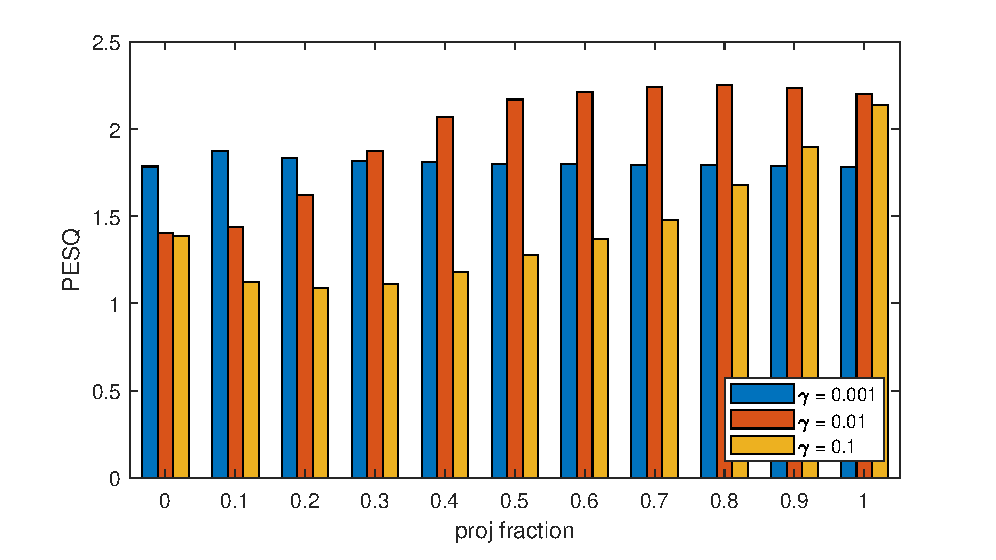
\includegraphics[width=1\linewidth]{figures/gamma_test}
	\caption{PESQ metric results made to choose the best value of $\gamma$ in DRA for testing with multiple audio files (these values are shown in the legend). 
		The results in terms of STOI and SNR were principally the same.
		The label \textit{proj fraction} refers to parameter $\beta$ from Alg.\,\ref{alg:DRA}.}
	\label{fig:gammatest}
	\vspace{-1em}
\end{figure}

We have chosen randomly 10 audio files for final evaluation from the Valentini dataset \cite{ValentiniBotinhao2017} described before.
As justified in \ref{subsec:soft_thresh}, we have chosen $\gamma = 0.01$.
The simulation was split to three restoration variants: two conventional ones and one including the learned denoiser.
The conventional ones were two versions of DRA \ref{alg:DRA} with same parameters except for the number of iterations ($50$ or $500$) and the choice of $\lambda_n$ (decreasing or constant).
The DRA with denoiser proposed in Alg.\,\ref{alg:pnp} was tested with $50$ iterations,
as in the shorter conventional method.
In all the algorithms, the initial $\lambda_0$ was set to $1$.
For the case of DRA \ref{alg:DRA} with 500 iterations, we kept constant $\lambda_n = 0.1$, which provided better results compared to the choice of $\lambda_n = 1$.
In the case of the plug-and-play version \ref{alg:pnp}, and the reference DRA \ref{alg:DRA} with 50 iterations, the parameter was set to decrease in every iteration as $\lambda_{n+1} = 0.9\cdot\lambda_n$.
The motivation for decreasing $\lambda$ is clear from Fig.\,\ref{fig:lamdadesc}.
The test was performed using DRA and every option should eventually converge to the same optimal point in time \cite{Combettes2011}.
However, the choice has an impact in practice, either in particular choice of the argument of the minima, or due to numerical reasons and finite number of iterations.
If $\lambda$ decreases, we minimize the impact of soft threshold operator in latter iterations which appears to be effective in our case.

\begin{figure}[!h]
	\centering
	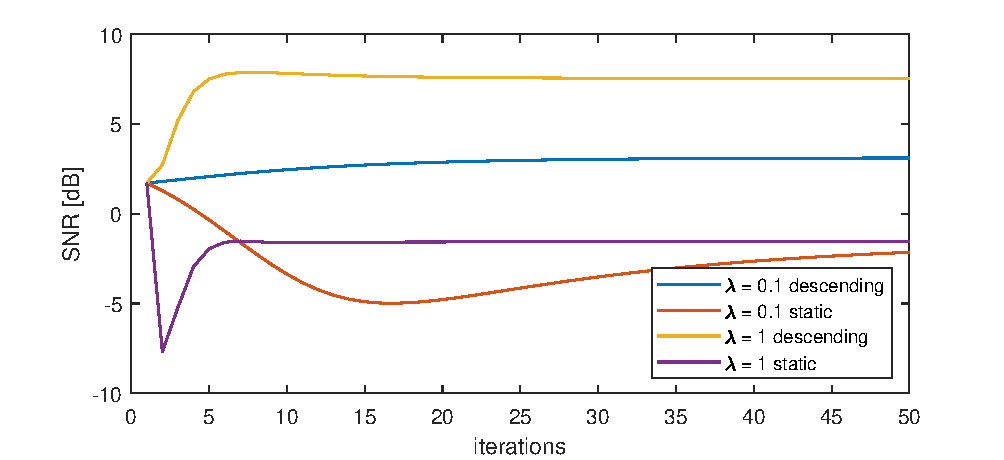
\includegraphics[width=1\linewidth]{figures/lamda_desc}
	\caption{SNR from DRA tested for 50 iterations with static and decreasing choice of $\lambda \in \{0.1,1 \}$.
	Tested signals are same as in experiment with $\gamma$.}
	\label{fig:lamdadesc}
\end{figure}




\begin{figure*}[t]
	\begin{subfigure}{.33\textwidth}
		\centering
		\includegraphics[width=1.1\linewidth]{figures/lam1_stoi}  
	\end{subfigure}
	\begin{subfigure}{.33\textwidth}
		\centering
		\includegraphics[width=1.1\linewidth]{figures/lam1_PESQ}  
	\end{subfigure}
	\begin{subfigure}{.33\textwidth}
		\centering
		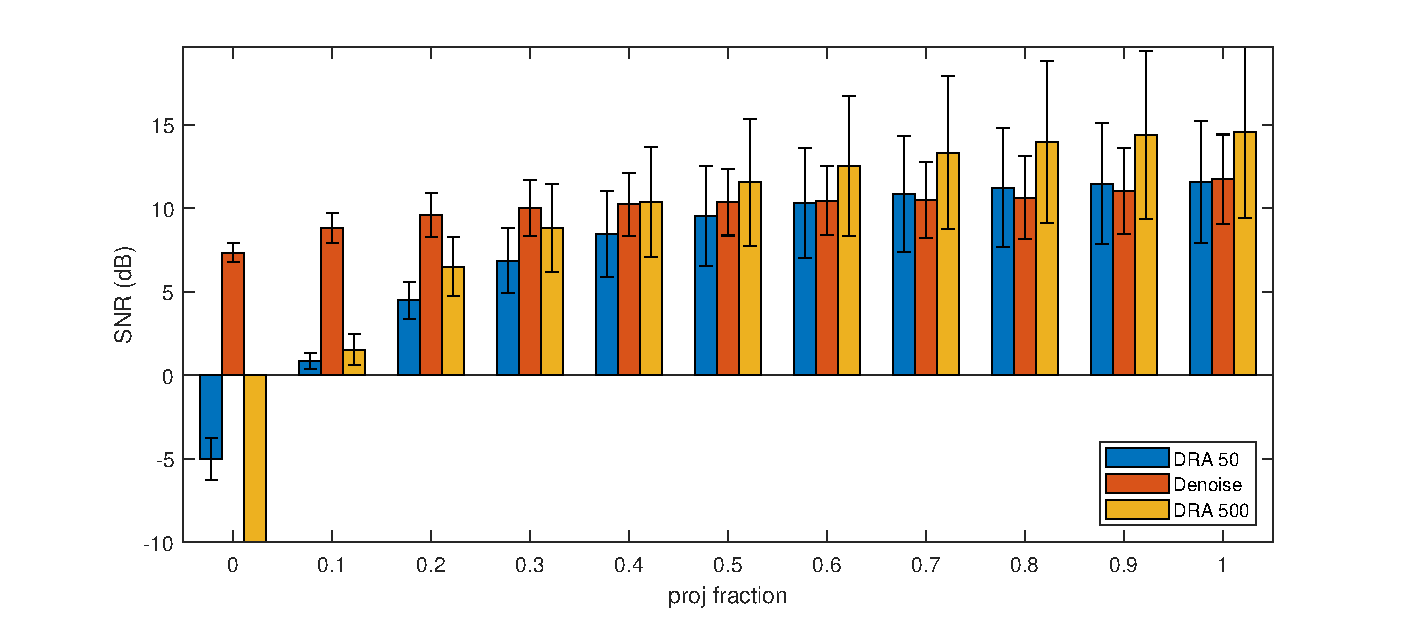
\includegraphics[width=1.1\linewidth]{figures/lam1_SNR}  
	\end{subfigure}
	\caption{Average results from 10 tested signals. Metrics are from left to right: STOI, PESQ, SNR.
		}
	\label{fig:final3witherrors}
\end{figure*}

\subsection{Comparison results}


Graphs with STOI, PESQ and SNR are presented in Fig.\,\ref{fig:final3witherrors}.
We see that plug-and-play is less sensitive to the fraction of projection compared to DRA,
and in comparison with DRA (50 iterations, decreasing $\lambda_n$), it reaches better result.
DRA with 500 iterations has higher variance of the results, but globally, it outperformed the plug-and-play method with optimal choice of the parameters such as the ratio $\beta$.




\section{Conclusion}
\label{sec:conclusion}

Our reformulation of plug-and-play method for audio inpainting with noisy data was demonstrated to be successful with properly chosen ratio of projection and $\lambda$.
Next steps could be to extend the test for other similar tasks (declipping, dequantization), following the pattern of root method \cite{Chan2016}, solving multiple tasks with one setup of the algorithm.
We also suggest suggested not to use off-the-shelf denoiser, but learn own model on data related to our problem (e.g.\ specific noise due to dropout of a certain percentage of samples).
In addition,
we might be able to make the self-learned denoiser non-expansive, thus satisfying the theoretical convergence guarantees \cite{Venkatakrishnan2013,Chan2016}.
A compromise might be to use transfer learning,
i.e., to take a successful denoiser and continue learning from a checkpoint with our dataset,
with idea to reduce artifacts generated in the inpainting task.


\bibliographystyle{IEEEtr}
\bibliography{bib_eeict2023}



\end{document}
